\documentclass[11pt]{article}
\usepackage[margin=1in]{geometry}
\usepackage[T1]{fontenc}
\usepackage{lmodern,amsmath,amssymb,amsthm,graphicx,booktabs,array}
\input{ot1lmr.fd}
\DeclareFontShape{OT1}{lmr}{m}{n}{<-> rm-lmr10}{}
\input{omllmm.fd}
\DeclareFontShape{OML}{lmm}{m}{it}{<-8.5> lmmi8 <8.5-> lmmi10}{}
\usepackage[numbers,sort&compress]{natbib}
\usepackage{enumitem,microtype,caption,fancyhdr}
\usepackage[colorlinks=true,linkcolor=black,citecolor=black,urlcolor=blue]{hyperref}
\hypersetup{pdftitle={Shaping Gap Benchmark: Effect Interfaces for Compositional Execution of Frozen Neural Computation},pdfauthor={Nathaniel Oh and Paul Attie}}
\usepackage{float,algpseudocode}
\floatstyle{ruled}\newfloat{algorithm}{tbp}{loa}\floatname{algorithm}{Algorithm}
\floatstyle{plain}
\setlength{\emergencystretch}{2em}
\setlength{\parskip}{0.2em}
\setlength{\headheight}{14pt}
\captionsetup{font=small,labelfont=bf}
\pagestyle{fancy}\fancyhf{}
\fancyhead[L]{\small Shaping Gap Benchmark}
\fancyhead[R]{}
\fancyfoot[C]{\thepage}
\newtheorem{proposition}{Proposition}
\newcommand{\R}{\mathbb{R}}
\newcommand{\silu}{\operatorname{SiLU}}
\newcommand{\rms}{\operatorname{rms}}
\newcommand{\eps}{\varepsilon}
\newcommand{\NativeSolved}{80}
\newcommand{\StructuredSolved}{129}
\newcommand{\DifferentialSolved}{104}
\newcommand{\ValueFewSolved}{100}
\newcommand{\ValueMatchedSolved}{105}
\newcommand{\RemovedSolved}{105}
\newcommand{\CorruptSolved}{108}
\newcommand{\TestConditions}{288}
\newcommand{\NativeReplays}{2592}
\newcommand{\BranchChecks}{512}
\newcommand{\SourceDirectionsChecked}{24}
\newcommand{\RestoredConditions}{288}
\newcommand{\StructuredSaving}{21.39}
\newcommand{\StructuredGain}{61.25}

\title{Shaping Gap Benchmark:\\Effect Interfaces for Compositional Execution\\of Frozen Neural Computation}
\author{Nathaniel Oh \and Paul Attie}
\date{November 12, 2026}
\begin{document}
\maketitle
\thispagestyle{plain}
\begin{abstract}
We introduce Shaping Gap Benchmark and a reference runtime for acquiring
reusable behavioral interfaces over native components of an ordinary frozen
pretrained model. The runtime uses those interfaces to construct computations
satisfying explicit neural requirements. An interface describes a
component's accumulated effect and how incoming context changes that effect.
Integrating this context sensitivity along a predecessor's displacement gives
a compatibility forecast for composition. The acquired descriptions persist
across requirements; the runtime constructs and deploys temporary native
programs from them. We implement source acquisition, bounded retained arrays,
compatibility-guided branching execution, and independent deployment.
A controlled study compares derivative-supervised quadratic acquisition,
endpoint-only acquisition, and a structure-calibrated reference across three
local activation domains and \TestConditions{} fresh numerical contracts.
The equal-context endpoint interface satisfies \ValueFewSolved{} contracts
versus \NativeSolved{} for local native sensitivity guidance, with 15.76\% less
acquisition-and-execution native-query work. Under the same online envelope,
the differential interface satisfies \DifferentialSolved{}, compared with
\ValueMatchedSolved{} for query-matched endpoint acquisition. Its context-partial
prediction improves in all three domains; conditioning removal and permutation
satisfy \RemovedSolved{} and \CorruptSolved{}, respectively, locating an
unresolved gap between predictive fidelity and construction benefit.
The structure-calibrated reference satisfies
\StructuredSolved{} with \StructuredSaving{}\% less source-and-execution
native-query work than local guidance. All \NativeReplays{} selected programs
replay exactly through original native components, with pretrained parameters
unchanged. A standalone structured representation additionally reproduces all
selected programs' contract decisions without loading the checkpoint, with
maximum readout error $3.31\times10^{-6}$.
The contribution is an acquired behavioral interface used as a construction
abstraction, together with a benchmark that measures its construction value
after acquisition and execution costs.
\end{abstract}

\section{Introduction}
A pretrained network supplies a large collection of learned computations.
Its original architecture gives one way to execute them. Recent work on
chain-of-layers and program-of-layers inference shows that frozen pretrained
layers can also be skipped, repeated, and recomposed into input-specific
programs \citep{cola,polar}. This makes an additional question concrete:
\emph{can reusable descriptions acquired from existing components improve
the cost of constructing computations that satisfy later requirements?}

We study \emph{effect-interface acquisition}. The runtime observes native
components, retains descriptions of their behavior, and uses those descriptions
to construct a computation satisfying an explicit neural contract. The contract
specifies which monitored responses should change and which should remain
within protected intervals. A constructed program is a sequence of original
components acting on live activation. Its execution is checked through the
original frozen parameters.

The key representation must describe more than a component in isolation.
Executing A changes the state in which B operates, including B's own neural
activity. A's immediate effect can therefore conceal a useful continuation,
or make an apparently useful B ineffective. Our interface pairs B's accumulated
effect $E_B$ with its incoming-context derivative $K_B=D E_B$. Integrating $K_B$
along A's displacement predicts how A conditions B. This turns compositional
compatibility into a measurable, context-dependent quantity.

The interface is the retained object. Its coefficients describe behavior across
source contexts and are reused under later contracts. The runtime uses them to
forecast alternatives, classify compatible continuations, execute proposed
native components, and deploy a selected program (Figure~\ref{fig:architecture}).
Acquisition and construction are consequently separate stages with separate
costs. In the present study, component boundaries, domains and monitored
readouts are supplied; the acquired content is their numerical behavior.

Shaping Gap Benchmark makes this question reproducible. It holds the frozen
component bank, requirements, native checker and online execution allowance
fixed, varies the source knowledge used by the construction engine, and charges
that knowledge's acquisition. The measured gap is a difference in achievable
contract satisfaction or cost over the same computational material. This first
study establishes the interface, its executable use, and its finite construction
frontier; the research program is to make acquisition itself a continuing
source of better constructions.

\begin{figure}[t]
\centering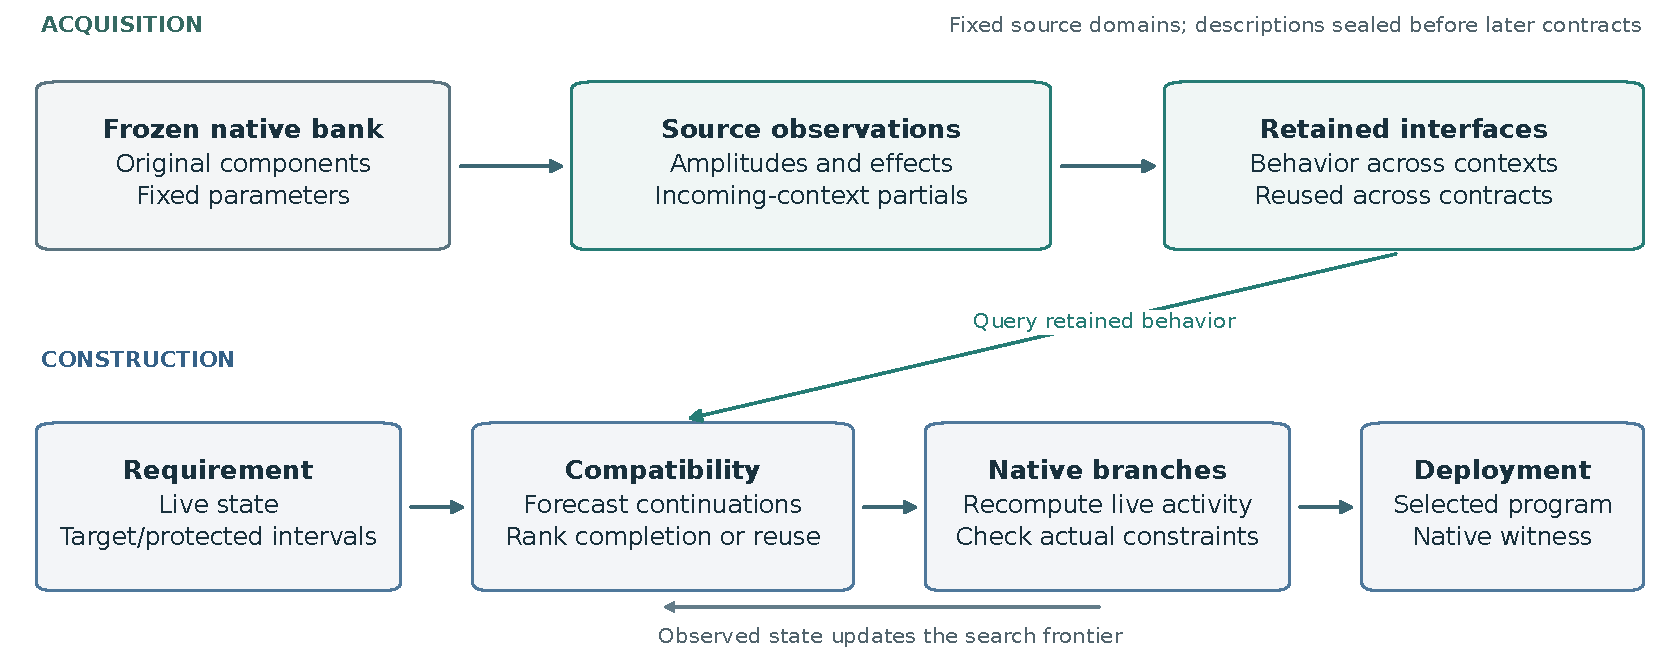
\includegraphics[width=\linewidth]{figures/interface-runtime.pdf}
\caption{The acquired interface connects frozen computational material to
requirement-guided construction. Source observations produce retained
descriptions before the later contracts are sampled. At runtime the live state
and contract query those descriptions; original native execution determines
the result. The interface persists across contracts, while the search frontier
and selected program belong to an individual construction.}
\label{fig:architecture}
\end{figure}

The study evaluates this separation directly. On \TestConditions{} fresh
numerical contracts, a 32-context endpoint interface satisfies
\ValueFewSolved{} versus \NativeSolved{} for online native local guidance,
with 15.76\% less total native-query work after acquisition. A reference supplied
with the native architectural form reaches \StructuredSolved{} with
\StructuredSaving{}\% less work. Derivative supervision improves incoming-context
prediction, but its extra conditioning term gives no net solve-count gain here.
The controls separate predictive fidelity, construction value and acquisition
return.

\begin{samepage}
Our contributions are:
\begin{enumerate}[leftmargin=*,itemsep=0.2em]
 \item An accumulated-effect/context interface that connects finite neural
       behavior to predecessor-conditioned composition, with conditional
       prediction and decision-stability bounds.
 \item A runtime that acquires and retains those descriptions, then uses them
       for compatibility-guided construction and deployment of original frozen
       components outside their original layer schedule.
 \item Shaping Gap Benchmark: an acquisition-inclusive study with matched-engine controls,
       conditioning interventions, complete native witnesses, and standalone
       replay of the finite structure-calibrated bank.
\end{enumerate}
\end{samepage}

The unit of retained learning is the behavioral interface; the unit of execution
is a temporary native program; the evaluation criterion is construction quality
against total charged work. This separation fixes the scope of the present
paper and the questions advanced by follow-on acquisition studies.

\section{Related work}
\paragraph{Programs over frozen pretrained layers.}
CoLa searches for input-specific chains of pretrained layers using skipping,
repetition and reordering \citep{cola}. PoLar subsequently learns a predictor
of layer-segment programs from valid programs collected by MCTS
\citep{polar}. These results establish alternative execution programs as a
practical use of frozen pretraining. Our runtime acquires component behavior
models and queries them under an explicit contract to forecast compositions.
The studied components are native SwiGLU atoms with live input-dependent
activities. Thus our organizing object is a reusable effect interface, while
PoLar's predictor learns a direct map from input to execution program.

\paragraph{Decomposition, recomposition and representation alignment.}
Kingetsu et al.\ learn supermasks that extract functional modules from a
trained classifier and recompose class subsets through mask unions and
confidence voting \citep{recomposition}. Model stitching and latent functional
maps connect representations from existing networks \citep{stitching,lfm}.
Deja Vu predicts contextual sparsity \citep{dejavu}; automatic circuit discovery
identifies influential subgraphs \citep{acdc}. These methods provide precedents
for exposing and reusing pretrained structure. We acquire predictive effects
of supplied native atoms and compose their state transformations to satisfy
new readout intervals. Table~\ref{tab:positioning} identifies the different
retained objects and construction decisions.

\paragraph{Neural program and skill libraries.}
Routing Networks, Neural Interpreters and Neural Attentive Circuits learn
modular execution \citep{routing,interpreters,nac}. HOUDINI uses types and
combinators to synthesize neural programs while learning their parameters
\citep{houdini}. DreamCoder and LILO acquire reusable program abstractions
\citep{dreamcoder,lilo}. Learned skill interfaces support planning over
continuous behavior \citep{skills,neuroskills}. We build on the idea that a
reusable description can make a component accessible to a planner. Here the
components come from an ordinary frozen pretrained model; the retained
description specifies their numerical effects and context sensitivity.

\paragraph{Model-based neural control.}
Activation-LQR uses layerwise local dynamics and reusable offline-computed
control gains to steer activations during inference \citep{alqr}. It supplies
a close precedent for amortizing knowledge of neural response. Our control
variable is a discrete native-component program. Its effect forecast includes
the successor's changed activity after a predecessor executes. The local
sensitivity baseline tests whether such retained descriptions help beyond
recomputing immediate native response at each search state.

\paragraph{Integrated derivatives and acquisition.}
Integrated Gradients accumulates response derivatives along paths; Integrated
Hessians measures pairwise feature interactions \citep{ig,ih}. Sobolev training
learns from function values and target derivatives \citep{sobolev}. These
provide the mathematical and approximation building blocks. Our interface
uses component execution and incoming state as its variables, and the runtime
uses the resulting description to forecast a construction. The study therefore
compares both prediction fidelity and its value in choosing executable programs.
The structure-calibrated reference separately measures the value of supplying
the known normalization and gating form.

\begin{table}[t]
\centering\small
\begin{tabular}{@{}>{\raggedright\arraybackslash}p{0.23\linewidth}>{\raggedright\arraybackslash}p{0.31\linewidth}>{\raggedright\arraybackslash}p{0.38\linewidth}@{}}
\toprule
Method & Reusable object & Execution decision\\
\midrule
PoLar \citep{polar} & Input-to-program predictor & Skip, keep or repeat layer segments\\[0.35em]
Module recomposition \citep{recomposition} & Learned class-subnetwork masks & Combine classifier modules\\[0.35em]
Activation-LQR \citep{alqr} & Control gains from local neural dynamics & Steer activations during layerwise inference\\[0.35em]
HOUDINI \citep{houdini} & Typed neural-function library & Synthesize and train a neural program\\[0.35em]
Our runtime & Native amplitude, accumulated effect and context partial & Forecast and construct a native program against a readout contract\\
\bottomrule
\end{tabular}

\caption{Methodological comparison. These works motivate the representation
and execution design; the numerical study compares our common-engine controls,
not performance on the cited works' application benchmarks.}
\label{tab:positioning}
\end{table}

\section{The interface and its compositional meaning}
\subsection{Construction problem and benchmark objective}
Let $\mathcal B=\{F_b\}$ be a supplied bank of frozen residual components,
$\Omega$ an activation domain and $q$ a supplied monitored readout. A later
requirement consists of an initial state $x\in\Omega$ and an interval contract
$C$ on selected coordinates of $q$. A program
$\pi=(b_1,\ldots,b_T)$ denotes
$F_\pi=F_{b_T}\circ\cdots\circ F_{b_1}$. Its success condition is
$q(F_\pi(x))\in C$, with the benchmark's numerical tolerance. Program depth
and the physical legality of every executed prefix are bounded by the declared
protocol.

Acquisition observes native behavior and retains interface parameters $\theta$.
Later construction queries $\theta$ under each requirement and explores
programs within an online native-query allowance. Native execution determines
success. The benchmark records the retained array payload, execution workspace,
native primitives and active time; each method's lifecycle includes its own
source acquisition and subsequent construction and deployment.

For a fixed ordered stream, let $S_j(c)$ be the number of contracts satisfied by
method $j$ after cumulative charged work $c$, counting unattempted contracts as
unsatisfied. The observed shaping gap between methods $i,j$ is
$S_i(c)-S_j(c)$; equivalently, one can compare work at the same attained count.
Acquisition is charged at the curve's origin. Native-query work and active time
give separate curves, since neither substitutes for the other. This definition
is an empirical construction frontier on the declared stream.

\subsection{Accumulated effect and the partial of that effect}
Let $x\in\R^d$ be live activation and $q:\R^d\to\R^m$ a fixed monitored neural
readout. Component $b$ is a compatible residual transformation
$F_b(x)=x+f_b(x)$, with fixed pretrained parameters. Its total effect is
\begin{equation}
 E_b(x)=q(F_b(x))-q(x)
       =\int_0^1 J_q(x+s f_b(x))f_b(x)\,ds .
 \label{eq:effect}
\end{equation}
The identity follows by differentiating $q(x+s f_b(x))$ with respect to $s$
and integrating coordinatewise. The path is an activation interpolation;
$s$ is not physical neural time or a trained weight.

Differentiating the accumulated effect with respect to incoming state gives
\begin{equation}
 K_b(x)=D_xE_b(x)=J_q(F_b(x))D_xF_b(x)-J_q(x).
 \label{eq:context}
\end{equation}
For a native atom $f_b(x)=D_ba_b(x)$, its complete derivative is
$D_xF_b=I+D_b\nabla a_b(x)^\top$. Thus $K_b$ includes the changed activity
of the successor itself. Holding its amplitude constant would omit a term.

For predecessor displacement $v$, define $G(\alpha)=E_b(x+\alpha v)$. Then
$G'(\alpha)=K_b(x+\alpha v)v$ and
\begin{equation}
 E_b(x+v)-E_b(x)=\int_0^1K_b(x+\alpha v)v\,d\alpha .
 \label{eq:conditioning}
\end{equation}
When $v=f_a(x)$, this is the finite interaction
\begin{equation}
 I_{a\to b}(x)=q(F_b(F_a(x)))-q(F_a(x))-q(F_b(x))+q(x).
 \label{eq:interaction}
\end{equation}
It differs from order dependence
$q(F_b(F_a(x)))-q(F_a(F_b(x)))$. A nonlinear readout can yield nonadditive
effects even for commuting fixed writes.

Equivalently, with
$Q(\alpha,\beta)=q(x+\alpha f_a(x)+\beta f_b(x+\alpha f_a(x)))$,
the derivative of B's accumulated effect is
$\partial_\alpha\int_0^1\partial_\beta Q\,d\beta$.
Under continuous mixed derivatives, integrating this quantity over $\alpha$
recovers the four-corner difference in Equation~\ref{eq:interaction}.
This closes the chain from local partials, to accumulated effect, to the
sensitivity of that accumulated effect.

\paragraph{Scope and trajectory information.}
The net effect in Equation~\ref{eq:effect} does not encode every intermediate
violation or turn. An interface may additionally retain applicability,
trajectory/protection evidence, uncertainty, and cost. The present central
experiment executes live-input components; a separate fixed root source would
require distinguishing incoming-state and root partials. We use real-arithmetic
smoothness for the identities and numerical validation for float32 execution.

\subsection{Conditional prediction and contract checking}
\begin{proposition}[Accumulated conditioning error]
Suppose $\|\widehat E_b(x)-E_b(x)\|\le\eps_E$ and
$\sup_{t\in[0,1]}\|\widehat K_b(x+tv)-K_b(x+tv)\|_{\rm op}\le\eps_K$.
Then
\[
 \left\|\widehat E_b(x)+\int_0^1\widehat K_b(x+tv)v\,dt-E_b(x+v)\right\|
 \le \eps_E+\eps_K\|v\|.
\]
\end{proposition}
\begin{proof}
Subtract Equation~\ref{eq:conditioning}, apply the triangle inequality,
and bound the integral by the operator-norm error times $\|v\|$.
\end{proof}
Quadrature error adds to this bound. An inaccurate predecessor displacement
also contributes its propagated error. Finite held-out mean error does not
establish the uniform premise.

\begin{proposition}[Robust interval margin]
If $|q_i-\widehat q_i|\le\eps_i$ and
$\ell_i+\eps_i\le\widehat q_i\le u_i-\eps_i$ for every monitored coordinate,
then $\ell_i\le q_i\le u_i$.
\end{proposition}
\begin{proof}
Combine the prediction margin and the coordinatewise error bound.
\end{proof}
The implementation uses predicted intervals to rank candidates and actual
native intervals to determine success. It does not treat an empirical error
statistic as a certified uniform margin.

\subsection{When an interface can determine a construction choice}
The composition identity makes the interface's role explicit:
\begin{equation}
 q(F_B(F_A(x)))-q(x)=E_A(x)+E_B(x+f_A(x)).
 \label{eq:composition}
\end{equation}
The second term is precisely the effect whose change is described by
Equation~\ref{eq:conditioning}. It is evaluated at the state produced by A.

Suppose the first displacement is approximated by $\widehat v$, and predict
the composed effect as
\[
 \widehat\Delta_{AB}=\widehat E_A(x)+\widehat E_B(x)
       +\int_0^1\widehat K_B(x+t\widehat v)\widehat v\,dt.
\]
If the two present-effect errors are at most $\eps_A,\eps_B$, the context
operator error is at most $\eps_K$ along the predicted path, and $E_B$ is
$L_B$-Lipschitz between $x+\widehat v$ and $x+f_A(x)$, then
\begin{equation}
 \|\widehat\Delta_{AB}-[q(F_B(F_A(x)))-q(x)]\|
 \le \eps_A+\eps_B+\eps_K\|\widehat v\|
          +L_B\|\widehat v-f_A(x)\|.
 \label{eq:pair-error}
\end{equation}
To obtain the bound, first apply the accumulated-conditioning bound along
$\widehat v$, then bound the change from its endpoint to the true endpoint.
Numerical quadrature contributes its own error. This separates immediate
effect fidelity, context fidelity and predecessor-amplitude fidelity.

\begin{proposition}[Compatibility decision stability]
Fix a nonempty finite set of physically admissible continuations $\Pi$ and a
nonempty closed interval contract $C$. Let
$d_C(q)=\inf_{c\in C}\|q-c\|_2$ and suppose
$\|\widehat q_\pi-q_\pi\|_2\le\eps$ for every $\pi\in\Pi$.
If $\widehat\pi$ minimizes $d_C(\widehat q_\pi)$ and $\pi^*$ minimizes
$d_C(q_\pi)$, then
\[
 d_C(q_{\widehat\pi})\le d_C(q_{\pi^*})+2\eps.
\]
If the true best continuation is unique and every alternative has a
distance gap greater than $2\eps$, the predicted choice equals the true best.
\end{proposition}
\begin{proof}
Distance to a nonempty closed set is 1-Lipschitz. Thus
$d_C(q_{\widehat\pi})\le d_C(\widehat q_{\widehat\pi})+\eps
\le d_C(\widehat q_{\pi^*})+\eps\le d_C(q_{\pi^*})+2\eps$.
A different selected continuation would contradict the stated gap.
\end{proof}
The search uses squared interval distance, which has the same minimizer.
This is a local choice guarantee on a fixed admissible set; native branching
checks physical feasibility. It suggests a decision-relevant acquisition
target: prediction accuracy relative to the separation between competing
continuations. Average held-out derivative error alone does not provide that
information.

\section{Native substrate and reachable coordinates}
We use the public four-bit MLX checkpoint of Qwen3-0.6B
\citep{qwen3,checkpoint,mlx}. A physical atom is an original SwiGLU neuron with
its original normalization, gate/up scalars and down-projection column:
\[
 a_b(x)=\silu((G_lN_l(x))_j)(U_lN_l(x))_j,\qquad
 f_b(x)=D_le_j\,a_b(x).
\]
These are actual native parameter-backed operations
\citep{rmsnorm,swiglu}. No fitted weights replace their execution. The loader
freezes the model and guards whole-model, transformer-block, attention,
embedding and unembedding calls. Original layer order is not a binding rule.

The fixed inventory has 22 physical units inherited from all producer
identities proposed in an earlier native pilot, including failures. Its
historical discovery work is charged. Native basis probes measure the output
directions, forming a full-column-rank matrix $D\in\R^{1024\times22}$.

\begin{proposition}[Reachable-coordinate closure]
If every update has the form $D e_b a_b(x)$, the
$b$th column of $D$ times $a_b(x)$, then executions beginning at
$x_0+Dz_0$ remain in $x_0+\operatorname{im}D$. In coordinates,
$z\mapsto z+e_ba_b(x_0+Dz)$, and
$D_zE_b(x_0+Dz)=K_b(x_0+Dz)D$.
\end{proposition}
\begin{proof}
Each update adds a column of $D$ times a scalar, so closure follows by
induction. The derivative statement is the chain rule.
\end{proof}
Float32 writes introduce small arithmetic residuals; native validation
checks actual arrays. We compute current coordinates with
$P=(D^\top D)^{-1}D^\top$. This is a supplied physical representation, not a
learned semantic vocabulary.

\section{Acquisition and intentional composition}
\paragraph{What is acquired and what is reused.}
For each supplied domain $\Omega$, component $b$ retains functions
$\widehat a_b(z)$ and $\widehat E_b(z)$, with context partial
$D_z\widehat E_b(z)$. These functions form its behavioral interface: the
amplitude determines a reachable displacement; the effect predicts a monitored
change; the context partial predicts how preceding computation changes that
effect. The same functions serve different target/protection masks and demands.
The later contract selects compatible continuations without refitting the
source model. Acquisition currently samples a supplied domain before those
contracts; the experiment does not learn the domain or the physical atom syntax.

The interface forecasts behavior, while the original component executes it.
An inaccurate forecast can therefore waste the search allowance, but final
success still requires a native execution witness. This division makes it
possible to test a representation's construction value independently of native
fidelity, and to charge source acquisition separately from repeated use.

\subsection{Generic acquired interfaces}
For each domain and component we observe its amplitude and accumulated
readout effect,
$y_b(z)=(a_b(x_0+Dz),E_b(x_0+Dz))$.
Native source derivatives supply both $\nabla_z a_b$ and $K_bD$.
The retained family is a generic quadratic:
\begin{equation}
 \widehat y_{b,r}(z)=c_{b,r}+L_{b,r}z+\tfrac12z^\top H_{b,r}z,
 \qquad H_{b,r}=H_{b,r}^\top .
 \label{eq:quad}
\end{equation}
It has 276 coefficients per scalar field. There are 22 amplitude fields and
$22\times12$ effect fields in each domain. Inputs are scaled by the declared
domain radius, outputs by source standard deviation with a fixed floor.

We fit ridge regression with source values and, for the differential arm,
their native coordinate derivatives. Value and derivative losses are averaged
over source contexts and derivative coordinates; both weights are one,
with ridge $10^{-6}$. Endpoint controls use the identical family and value
loss. No feature or regularization selection uses later results.

The polynomial's derivative and its directional integral are consistent:
\[
 \widehat y_b(z+te_a)-\widehat y_b(z)
 =t\,\partial_a\widehat y_b(z)+\tfrac12t^2(H_b)_{aa}.
\]
Consistency describes the retained approximation; source and held-out native
observations determine its fidelity to the component.

\subsection{Structure-calibrated reference}
We also supply a reference with the known RMSNorm/SwiGLU form. A normalized
linear scalar $g(x)=Ax/r(x)$ satisfies
$A=rJ_g+gx^\top/(d\,r)$ at a calibration anchor. Native partials therefore
recover the needed row restricted to the reachable directions.
For $x=x_0+Dz$,
\[
 r(z)^2=\|x_0\|^2/d+2x_0^\top Dz/d+z^\top D^\top Dz/d+\eps .
\]
Gate, up and readout numerators are affine in $z$. Original SwiGLU scalars
then define component amplitudes and composed effects in reduced coordinates.
Calibration costs 113 linear-projection equivalents per domain. This reference
receives architectural structure that the generic quadratic learner does not;
its source cost and accuracy are reported rather than assumed.

\subsection{Compatibility forecasting and native search}
For candidate A, let $t=\widehat a_A(z)$. The engine predicts A's effect and
integrates each successor's context sensitivity along $te_A$:
\[
 \widehat E_{B|A}
 =\widehat E_B(z)+t\,\partial_A\widehat E_B(z)
       +\tfrac12t^2(H_B)_{AA}.
\]
It forecasts the composed readout from
$q+\widehat E_A+\widehat E_{B|A}$. The best compatible successor defines a
context/requirement-dependent class for A. Classes therefore arise from
predicted composition, rather than fixed semantic names or round-robin
cluster quotas.

The common beam engine retains alternative partial native graphs. It permits
temporary loss increases and protected-coordinate excursions, while enforcing
the physical activity, write, state and domain limits on every actual branch.
A native checker determines final interval satisfaction. At each node the
ranking can stop after a predicted one-step completion or forecast a successor.
Only one-step guidance is used at the final depth or insufficient remaining
allowance. Successful or best selected graphs are independently deployed from
their original input with native activities recomputed.

\begin{algorithm}[t]
\caption{Acquire, classify, construct, and deploy}
\begin{algorithmic}[1]
\State Measure physical ports and define the compatible reachable domain
\State Observe source native amplitudes, accumulated effects, and context partials
\State Fit and retain scoped interfaces; seal their bytes before later requirements
\For{each later requirement}
 \State Initialize the native activation frame and bounded search frontier
 \While{frontier, depth, and query allowance permit}
  \State Forecast predecessor-conditioned successor effects from retained interfaces
  \State Classify compatible continuations; rank completion or continuation
  \State Execute proposed native components and check actual physical limits
  \State Update the frontier with observed states; recognize native final success
 \EndWhile
 \State Deploy the selected graph; release temporary search states
\EndFor
\end{algorithmic}
\end{algorithm}

\section{Central experimental design}
\paragraph{Domains and requirements.}
Three fixed anchors have RMS amplitudes 0.12, 0.25 and 0.6, with consumer layers
14, 20 and 25. Each uses 12 native gate coordinates sampled from anchor values
whose absolute magnitude lies in $[0.05,2]$. Source latent coordinates are
uniform in $[-1.5,1.5]^{22}$; later initial coordinates are uniform in
$[-0.5,0.5]^{22}$. Later components read live state.

For each of \TestConditions{} fresh contexts, six readout roles are sampled:
three must increase by a fixed cohort demand, and three must remain within
$\pm0.05$ of their initial values. Four ordered cohorts use increases
0.025, 0.05, 0.075 and 0.1. Each cohort contains 24 fresh contexts per domain.
The checker allows $10^{-5}$ numerical violation. Native amplitude is bounded
by 2, write RMS by 0.15, live RMS by 2, and latent coordinates by the domain.

\paragraph{Source and controls.}
Differential acquisition observes 32 contexts per domain. The equal-context
endpoint control sees those same value observations. A query-matched endpoint
control sees 347 contexts: 22,555 versus 22,560 source LPE per domain.
Eight additional contexts per domain diagnose fidelity without model selection.
All source objects are sealed before later outcomes.

Nine arms share the same six-depth, four-wide, six-child search engine. They
use native local sensitivity, equal-context endpoints, query-matched endpoints,
differential paired forecasts, differential one-step forecasts, conditioning
removed, conditioning permuted, restored conditioning, or the structured
reference. Removing conditioning preserves present effects. Permutation
changes the incoming direction associated with each conditioning operator;
restoration returns the exact original interface.

\paragraph{Protocol revision and chronology.}
A first registered batch, P46, completed 288 cases. Code review identified
that its paired forecast lacked an explicit terminal option and used two-step
ranking at the final depth. The correction was applied symmetrically to all
paired arms. P47, the reported final comparison, uses 288 fresh latent
contexts and masks with every source model byte unchanged. P46 remains in the
record as development; its outcomes are not pooled into the final rate.

\paragraph{Resource envelope.}
Each search has 512 LPE: a forward native linear projection counts one;
the corresponding input-adjoint projection counts one. A native producer
gradient has two reverse projections. Norm and scalar work are recorded
separately. LPE is an explicit native-query proxy, not a hardware FLOP or
energy unit. Scalar planning, fitting, logging and allocation appear in active
wall measurements. The retained interface/coordinate payload is bounded by
8\,MiB and the producer-activity cache by 1\,MiB; full process memory is
reported separately.

The lifecycle ledger includes historical inventory discovery, new physical
ports and domain setup, required source acquisition and fitting, all search
queries, and selected-graph deployment. Validation and independent scientific
replay are separately itemized research expenses. The 32-context endpoint source wall
cost is measured by a separate exact source-only replay, rather than inferred
by proportionally dividing the larger source time. All solver arm orders
rotate deterministically across cases.

\section{Results}
\subsection{Construction frontier and lifecycle cost}
Table~\ref{tab:main} reports the complete final comparison. The learned
differential interface satisfies \DifferentialSolved{} of \TestConditions{}
conditions, compared with \NativeSolved{} for native local guidance and
\ValueFewSolved{} for equal-context endpoint acquisition. The query-matched
endpoint control satisfies \ValueMatchedSolved{}.

\begin{table}[t]
\centering\small
\begin{tabular}{lrrrr}
\toprule
Method & Solved & Source LPE & Lifecycle LPE & Active s\\
\midrule
Native local & 80 & 0 & 130,416 & 26.55 \\
Endpoint, 32 contexts & 100 & 6,240 & 109,865 & 27.94 \\
Endpoint, query-matched & 105 & 67,665 & 173,739 & 39.77 \\
Differential interfaces & 104 & 67,680 & 173,016 & 34.54 \\
Differential, one-step & 102 & 67,680 & 173,487 & 33.95 \\
Conditioning removed & 105 & 67,680 & 172,401 & 34.18 \\
Conditioning permuted & 108 & 67,680 & 172,497 & 34.26 \\
Restored & 104 & 67,680 & 173,016 & 34.50 \\
Structured reference & 129 & 339 & 102,519 & 27.38 \\
\bottomrule
\end{tabular}

\caption{Final comparison. Source LPE excludes common inventory/port work;
lifecycle LPE includes it, source acquisition, search and all selected-graph
deployment. Active wall includes measured source fitting and CPU planning.
All rows use the same online envelope and native quality checker.}
\label{tab:main}
\end{table}

The structured reference is strongest: \StructuredSolved{} conditions versus
\NativeSolved{} for native local guidance, with \StructuredSaving{}\% less
lifecycle query work. The 32-context endpoint pipeline also increases solve count while
reducing this work. These gains concern interface-guided construction under the
declared query metric. Their active-wall advantage differs: source acquisition,
Python planning, and native kernels have different costs.

\begin{figure}[t]
\centering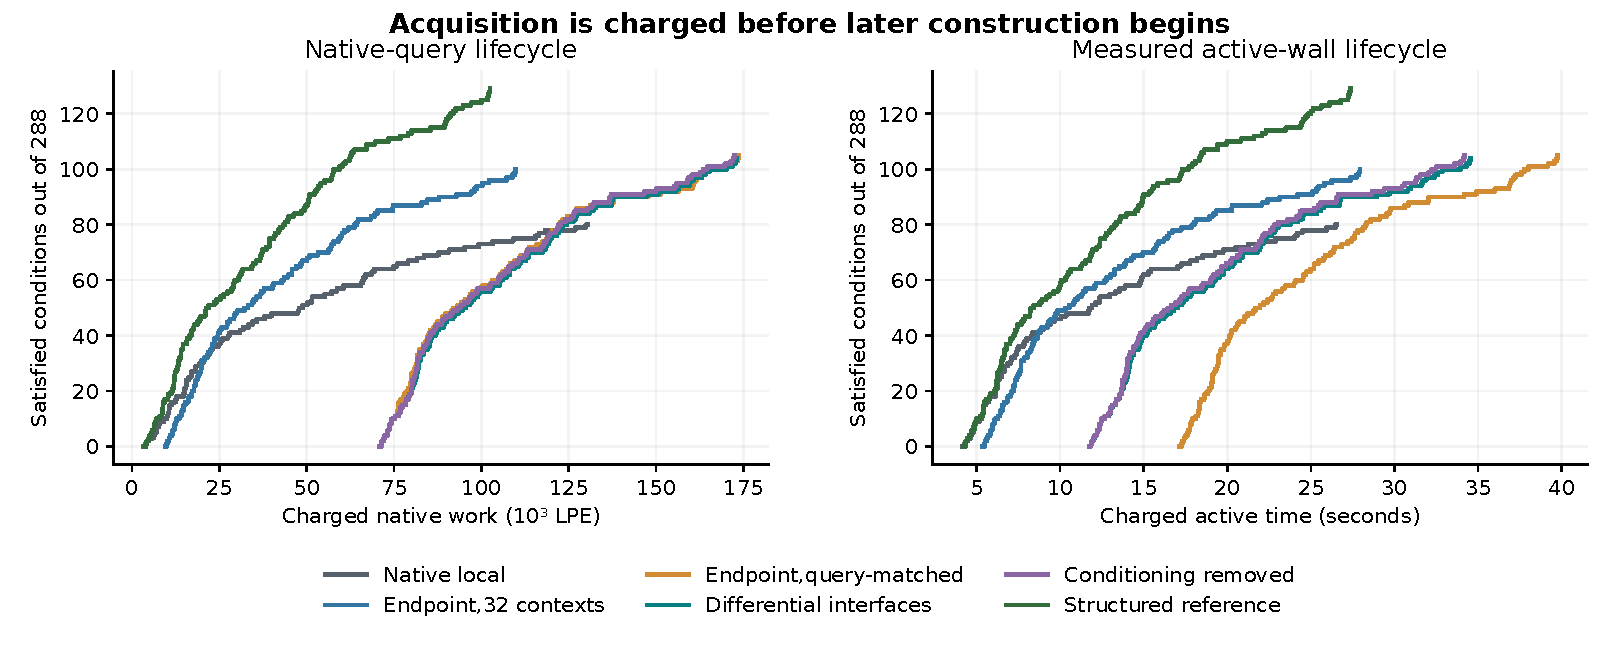
\includegraphics[width=\linewidth]{figures/lifecycle.pdf}
\caption{Cumulative fixed-stream quality with acquisition charged at the origin.
The two axes expose different resource tradeoffs. Unattempted conditions count
as unsolved under an interrupted stream. These curves do not replace paired
per-condition outcomes or imply that LPE equals wall time.}
\label{fig:lifecycle}
\end{figure}

At the common 102,519-LPE stream budget, native local guidance has satisfied
73 conditions, 32-context endpoint has 96, the differential pipeline has 56, and the
structured reference has 129. The differential acquisition overhead has not
amortized against the local baseline under that query budget. At the common
26.55-second active-wall budget, the respective counts are 80, 96, 87, and
124. The source-and-execution ledger is therefore essential to interpreting
online query gains.

\subsection{Context sensitivity and its causal use}
Differential supervision improves held-out $K$ fidelity in each domain,
including against the query-matched endpoint learner. Its total-effect
prediction does not dominate the query-matched control
(Table~\ref{tab:validation}). Approximation quality also varies sharply with
domain scale.

\begin{table}[t]
\centering\small\begin{tabular}{lrrrr}
\toprule
\multicolumn{5}{c}{Accumulated effect $E$: RMSE}\\
Domain & Differential & Endpoint32 & Query-matched & Structured\\
\midrule
1 & 0.3573 & 0.3605 & 0.3359 & 4.727e-07 \\
2 & 0.1801 & 0.2486 & 0.162 & 5.653e-07 \\
3 & 0.006823 & 0.04174 & 0.006529 & 7.392e-07 \\
\midrule
\multicolumn{5}{c}{Context partial $KD$: RMSE and native scale}\\
Domain & Differential & Endpoint32 & Query-matched & Native RMS\\
\midrule
1 & 0.1164 & 0.1242 & 0.1416 & 0.129 \\
2 & 0.05316 & 0.06347 & 0.06057 & 0.06796 \\
3 & 0.002309 & 0.01196 & 0.002697 & 0.01451 \\
\bottomrule
\end{tabular}

\caption{Held-out effect and reachable-coordinate context-partial RMSE on
eight native contexts per domain, each with 22 components and 12 readouts.
The lower panel's final column gives the native partial's RMS scale.
Coordinates and bindings sharing a context are correlated; they are not
independent task trials.}
\label{tab:validation}
\end{table}

Conditioning removal changes 45 selected graphs and satisfies
\RemovedSolved{} conditions; permutation changes 45 graphs and satisfies
\CorruptSolved{}. Against removal, full conditioning wins one case and loses
two; against permutation it wins one and loses five. Restoring the interface
reproduces all \RestoredConditions{} graphs and final states exactly.
Thus conditioning participates in construction, but its incremental solve-count
benefit is absent in this realization. Against one-step use of the same
differential interface, paired use wins six cases and loses four.

\begin{table}[t]
\centering\small\begin{tabular}{lrrrr}
\toprule
Method & Domain 1 & Domain 2 & Domain 3 & Total\\
\midrule
Native local & 15 & 36 & 29 & 80 \\
Endpoint,32 contexts & 4 & 50 & 46 & 100 \\
Endpoint,query-matched & 7 & 50 & 48 & 105 \\
Differential interfaces & 5 & 51 & 48 & 104 \\
Differential,one-step & 6 & 48 & 48 & 102 \\
Conditioning removed & 7 & 50 & 48 & 105 \\
Conditioning permuted & 9 & 51 & 48 & 108 \\
Structured reference & 28 & 53 & 48 & 129 \\
\bottomrule
\end{tabular}

\caption{Satisfied conditions by domain, 96 per column. Heterogeneity matters:
a global quadratic is substantially less faithful in the highest relative
perturbation domain.}
\label{tab:domains}
\end{table}

The data distinguish three contributions that should not be conflated:
reusable source-derived behavior, multi-step compatibility forecasting, and
the learned conditioning increment. Their costs and ablations differ.

\subsection{Native fidelity and validation}
All \NativeReplays{} selected programs were independently replayed in a fresh
process through the original full hidden activity and masked native
down-projection. Full final activation/readout arrays and interval decisions
match bit for bit. A deterministic reservoir of \BranchChecks{} branches
checks parent reconstruction, activity, physical legality, write and readout.
All original parameter bytes remain unchanged.

Twenty-four source directional derivatives were additionally checked against
direct autodiff of the complete native component/readout program. An initial
central-difference step of 0.005 passed 17 of 24 prescribed tolerance checks.
The preserved step sweep passes 24 of 24 at 0.02 and worsens as the step shrinks
to 0.001 and 0.0002, consistent with cancellation of small effect differences
in float32. Direct program autodiff passes all 24 directions. Both the initial
failures and the convergence data remain in the evidence record.

The final evaluation process peaks at approximately 530\,MiB RSS, including
the full frozen checkpoint. Retained quadratic interface/coordinate arrays
occupy 3,852,784 bytes across three domains; the structured reference occupies
415,840 bytes. These are logical array payloads, not complete Python or
training-workspace memory bounds.

\paragraph{Standalone execution of the acquired bank.}
We replayed every selected program using the structured representation in a
separate NumPy-only process that neither imports MLX nor opens the checkpoint.
It recomputes every live component amplitude in reachable coordinates.
All 2,592 contract decisions agree with the recorded native decisions; maximum
absolute readout error is $3.3021\times10^{-6}$. The structured formulas occupy
43,104 array bytes across three domains, or 415,840 bytes including output
directions, input coordinate projection and anchors. This payload represents
the finite 22-unit bank and its fixed monitored readouts. The replay process
peaks at 61,702,144 bytes RSS. Its 0.822-second replay measurement includes
reading the case-root arrays; it is not a matched native-kernel speedup
comparison. This checks that the interface can be executable computational
material, rather than only a ranking annotation.

\section{Interpretation and scope}
The central result is that effect-interface acquisition can make frozen native
components usable in a different compositional execution regime, with explicit
resource and fidelity checks. The structured reference demonstrates the value
of supplying an accurate behavioral representation. Generic endpoint learning
also improves the measured construction frontier relative to online local
sensitivity.

The contribution connects reusable description to executable composition.
Related methods establish layer programs, extracted modules and neural control;
our runtime retains a model of what native components do in context and queries
it under each new contract. The source object is reused across requirements,
while construction can select a different native program each time. The
standalone finite-bank replay further shows that an accurate acquired
representation can carry executable behavior as well as guide original-native
construction.

Derivative-supervised acquisition supplies more accurate context sensitivities,
but the present conditioning forecasts do not improve net construction over
their removal or permutation. The error bound explains why average derivative
fidelity is insufficient: planning needs accurate effects and conditioning along
the relevant displacement, at margins small enough for the requirement.
Equation~\ref{eq:pair-error} identifies the prediction terms that matter, and
the decision-stability proposition ties their combined error to the separation
between continuations. This identifies the next acquisition target:
context-scoped interfaces whose task-relevant effects and conditioning are
reliable where compatibility decisions change.

Three design extensions follow directly. Acquisition can concentrate on native
construction blockers rather than uniform domain coverage. A local or adaptive
representation can replace a single global quadratic where curvature is large.
Regression control can learn when an acquired operator is applicable rather
than applying it indiscriminately. Each extension should retain the same
execution engine and full cost comparisons.

The mathematical formulation applies to compatible differentiable component
maps; the empirical study covers one checkpoint, a finite unit bank and supplied
numerical readouts. Pretraining-specific advantage over random weights is not
isolated. Meaningful semantic contracts, larger inventories, attention fragments,
cross-model transfer and repeated acquisition cycles are further evaluations.
The present reuse stream measures amortization opportunity, rather than continual
compounding across interface revisions.

\paragraph{Lifecycle criterion.}
For stationary costs, acquisition $C_A$ amortizes against old per-use cost $C_0$
only when $C_A+n(C_1+C_M)<nC_0$, where $C_1$ is new execution and $C_M$
maintenance. If $C_0>C_1+C_M$, break-even requires
$n>C_A/(C_0-C_1-C_M)$. The study instead reports cumulative measured curves,
because demands and success vary. Acquisition, storage, prediction and
maintenance are part of the method's resource claim.

\section{Research program}
The present paper establishes a common object, runtime and measurement protocol
for studying acquired access to frozen computation. The next stages ask how
that access can become more useful, accumulate under a budget, and support
capabilities with external meaning. Each stage should keep the source knowledge,
construction procedure and lifecycle accounting explicit.

\paragraph{Decision-relevant acquisition.}
Which native observations should the system acquire next? The composition-error
bound separates effect, context and displacement errors; compatibility stability
depends on those errors relative to the separation between continuations. This
suggests acquiring distinctions where a construction decision is unresolved,
with local applicability and calibrated uncertainty. The empirical test is
whether targeted acquisition improves later native construction enough to
repay its additional observations, against fixed-data and equal-work controls.

\paragraph{Continual acquisition and consolidation.}
Can a sequence of solving, acquiring descriptions, consolidating and reusing
them reduce the cost of acquiring subsequent capabilities? This requires
repeated interface revisions, not just reuse of one sealed source fit.
Comparisons should include fixed and extract-once repertoires under matched
retained-state and active-workspace limits. Failed acquisitions, consolidation,
eviction, rediscovery and regression checks belong in the same cost ledger.
The target is a sustained improvement in later cost-to-quality as demand rises,
measured against those controls over a declared horizon.

\paragraph{Broader capability and resource scaling.}
How can internally recognizable contracts be grounded in externally useful
capabilities? This stage connects native construction to externally checked
tasks, expands component banks and readouts, and repeats the method across
pretrained architectures. Random or otherwise matched substrate controls can
isolate the contribution of pretraining. Active footprint, retained state,
total computation and latency should be measured separately as demand grows.
These experiments would test how far improved organization can substitute for
additional resources in a concrete application.

The long-term objective is a system whose accumulated descriptions of frozen
computation support progressively more capable executable organizations within
a bounded active envelope. Shaping Gap Benchmark supplies a starting point:
explicit native contracts, acquired behavioral interfaces, executable witnesses
and a shared acquisition-inclusive criterion for judging each subsequent step.

\section{Conclusion}
We introduced Shaping Gap Benchmark and a runtime that acquires reusable behavioral interfaces over
ordinary frozen pretrained components and uses them to construct native
programs satisfying explicit neural requirements. Accumulated effects describe
what a component changes; incoming-context partials describe how predecessors
change that effect. Together they give the runtime an operational description
for composition, with conditional error and decision-stability guarantees.

The study connects this representation to native witnesses and acquisition-
inclusive lifecycle curves. Endpoint interfaces improve the measured
construction frontier; structure calibration gives the strongest result.
Derivative supervision improves context prediction, while the present
conditioning policy adds no net solve-count benefit. These results make the
next mechanism concrete: acquire behavioral knowledge with sufficient
decision-relevant precision to make later constructions reliably cheaper.

\bibliographystyle{plainnat}
\bibliography{references}

\appendix
\section{Artifact and experimental chronology}
The physical inventory was fixed before the present source acquisition. It
contains all 22 producer identities proposed by an earlier native calibration,
including failed proposals. Its historical discovery work is charged to every
method. The artifact records both the inventory and its inherited cost receipt.

The source-acquisition batch (P46) measures native directions, samples the three
source domains, fits the interface controls, calibrates the structured reference
and seals their arrays. Its eight validation contexts per domain are diagnostic.
The subsequent development constructions exposed the missing terminal option
in paired forecasts. The same stop-aware correction was then applied to all
paired controls before the final batch (P47), which uses 288 fresh states and
masks. The final study reuses every sealed source-model byte and does not pool
the development outcomes into its comparison.

The supporting artifact links protocols, source arrays, selected programs and
cost receipts to the reported tables. It also preserves the original numerical
verification history: the failed small-step finite-difference check, the step
sweep and the final direct-autodiff checks.

\section{Recorded reproducibility boundary}
The checkpoint revision is
\texttt{173234aa840d113125e9f2271100ddbaf16c9620}.
The loaded stored-parameter SHA-256 is
\begin{center}\small\ttfamily
27a04e3e5e6b1d524751fa34d1053044bce9\\
ce7e4995e5b63b5c6b2a2dfe3798
\end{center}
The recorded environment uses NumPy 2.5.4, MLX 0.32.4 and MLX-LM 0.32.2
on the local Apple Metal runtime. Parameter bytes total 316,747,776.
Native bitwise replay is a statement about this recorded runtime; it does not
assert cross-device determinism.

The evidence package retains registered local protocols, exact runner/helper
snapshots, source arrays and interface coefficients, all case roots, complete
primitive/branch records, failed verification receipts, source derivative
convergence, final native verification, cost ledgers and evidence-derived
tables. Full checkpoint files are excluded; acquired interfaces and derived native
observations are included.
The companion repository URL is
\url{https://github.com/calysteon/shaping-gap-benchmark}. It includes the paper
and its source, portable experiment entry points, pinned source observations,
contracts, selected programs and result receipts. Fresh native runs regenerate
complete primitive and branch traces.

\subsection{Inventory and prospective seeds}
The physical inventory is recorded below. IDs are original layer/neuron
coordinates, not authored operation labels.
\begin{center}
\small
\begin{tabular}{rl}
\toprule
Layer & Neuron indices\\
\midrule
6 & 2069\\
10 & 211\\
13 & 573\\
16 & 2273\\
18 & 74, 804, 1234, 1741, 1839, 2230, 2465, 2490, 2599\\
19 & 622, 2864\\
20 & 2602\\
21 & 2259, 2386\\
23 & 1226\\
24 & 1914, 2701\\
\bottomrule
\end{tabular}
\end{center}
Anchor seeds are 61001--61003, readout-selection seeds 61501--61503,
source seeds 62001--62003 and validation seeds 63001--63003. The fixed
endpoint budget selects the first 347 source draws; the differential arm uses
the first 32. P46 uses later seeds 64001--64288 and P47 uses 66001--66288.
Requirement masks use each later seed plus 900000. The direction-permutation
control uses seed 65001. NumPy's recorded default generator produces all draws.

The host is an Apple M4 Max with 36\,GiB physical memory. Timing values are
single recorded runs with deterministic arm-order rotation; the study reports
paired outcomes and complete query counts alongside those measurements.
The compact reproduction package contains acquired arrays, code, protocols
and case roots. Full primitive/branch traces are retained separately, with
content hashes connecting them to the results.
\end{document}
